\section{Auswertung}
\label{sec:auswertung}

Im Folgenden werden die aufgenommenen Messdaten ausgewertet, um den Kernspin der Isotope zu bestimmen.
Dafür müssen zunächst die Landé-Faktoren der Isotope bestimmt werden und die vertikale Komponente des Erdmagnetfeldes.
Anschließend wird das Isotopenverhältnis der Rubidium-Isotope bestimmt und der quadratische Zeeman-Effekt untersucht.

Es werden die Werte der Magnetfeldstärken der Horizontalen Spule berechnet, indem die jeweiligen Anteile der sweep und der
horizontalen Verschiebungsspule addiert werden.
Für die Magnetfeldstärken der Spulen im Zentrum gilt

\begin{equation}
    B(0) = \frac{8  \mu_0  N I}{\sqrt{125} A}  \, .
    \label{eqn:magnetfeld}
\end{equation}

Die Stromstärke des Sweepanteils wird per Umdrehnungen gemessen.
Dieser Wert wird mit \qty{0.1}{\ampere} pro Umdrehung umgerechnet.
Für den horizontalen Anteil wurde die Spannung in \unit{\milli\volt} gemessen und kann umgerechnet werden in \unit{\milli\ampere},
indem die Werte der Spannungen verdoppelt werden.
Die notierten Werte werden in Tabelle \ref{tab:magnetfeldstärken} aufgetragen, wobei die Stromstärken bereits umgerechnet wurden.

\begin{table}
    \centering
    \caption{Die aufgenommenen Messwerte der Sweep-Spule und der horizontalen Verschiebungsspule für beide Isotope.}
    \label{tab:magnetfeldstärken}
    \begin{tabular}{c c c c c}
        \toprule
        $f \mathbin{/} \mathrm{kHz} $& $I_{s1} \mathbin{/} \unit{\ampere}$ & $I_{h1} \mathbin{/} \unit{\ampere}$ & $I_{s2} \mathbin{/} \unit{\ampere}$ & $I_{h2} \mathbin{/} \unit{\ampere}$ \\
        \midrule
        100 & 0.54 & 0.00 & 0.658 & 0.00 \\
        200 & 0.776 & 0.00 & 0.731 & 0.0194 \\
        300 & 0.436 & 0.0402 & 0.790 & 0.0402 \\
        400 & 0.328 & 0.0642 & 0.801 & 0.0642 \\
        500 & 0.291 & 0.0834 & 0.891 & 0.0834 \\
        600 & 0.281 & 0.1006 & 0.987 & 0.1006 \\
        700 & 0.10 & 0.1298 & 0.928 & 0.1298 \\
        800 & 0.272 & 0.1374 & 0.433 & 0.1894 \\
        900 & 0.384 & 0.1432 & 0.598 & 0.2028 \\
        1000 & 0.459 & 0.2374 & 0.522 & 0.2328 \\
        \bottomrule
    \end{tabular}
\end{table}

In Abbildung \ref{fig:plot1} sind die mit der Gleichung \ref{eqn:magnetfeld} berechneten Magnetfeldstärken gegen die Frequenz für beide Isotope aufgetragen.

\begin{figure}
    \centering
    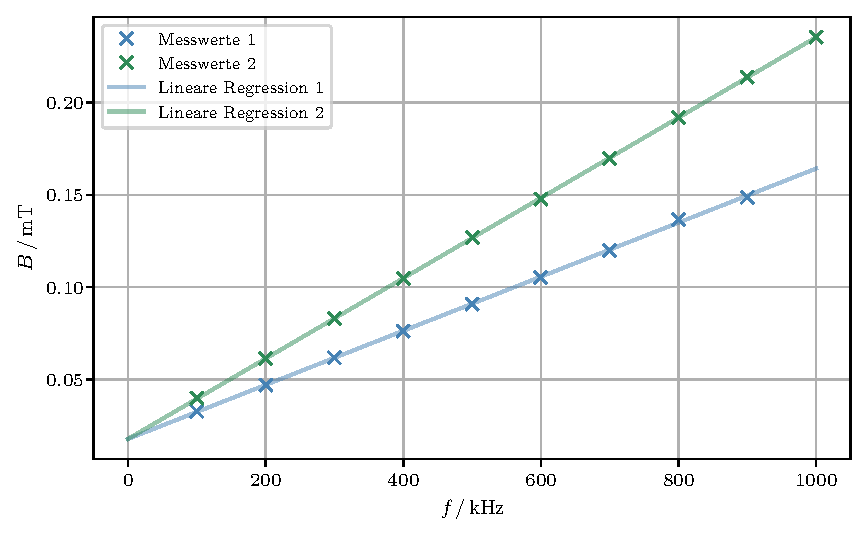
\includegraphics[width=0.8\textwidth]{build/plot.pdf}
    \caption{Magnetfeldstärke aufgetragen gegen die Frequenz für beide Isotope.}
    \label{fig:plot1}
\end{figure}

Es wurde eine lineare Regression der Messwerte für beide Isotope durchgeführt.
Die verwendete Ausgleichsfunktion hat die Form
\begin{equation}
    f(x) = a \cdot x + b \, .
\end{equation}

Daraus folgen die Parameter beider Isotope
%a_1: (1.468+/-0.011)e-07
%b_1: (1.76+/-0.06)e-05
%a_2: (2.1795+/-0.0035)e-07
%b_2: (1.760+/-0.022)e-05

\begin{align*}
    a_1 &= \qty{1.468(11)e-07}{\tesla\per\hertz} \\
    b_1 &= \qty{1.76(6)e-05}{\tesla} \\
    a_2 &= \qty{2.1795(35)e-07}{\tesla\per\hertz} \\
    b_2 &= \qty{1.760(22)e-05}{\tesla} \, .
\end{align*}

Die berechneten Werte werden für die weiteren Rechnungen verwendet

\subsection{Magnetfeld der Erde}
\label{sec:magnetfeld-der-erde}

Die Vertikalkomponente des Erdmagnetfeldes hat aufgrund des horizontal verlaufenden Lichtstrahls einen Einfluss auf die Messung.
Daher wird diese durch ein vertikal verlaufendes Magnetfeld kompensiert und der Aufbau wird um die vertikale Achse in Nord-Süd Richtung gedreht,
sodass die horizontale Komponente parallel oder antiparallel zu dem horizontalen Magnetfeld verläuft.
Zur Berechnung der Feldstärke des Erdmagnetfeldes muss zunächst die magnetische Feldstärke des vertikalen Feldes gemessen werden.
Diese betrug in diesem Experiment \qty{0.23}{\ampere}.
Anschließend wird über den $y$-Achsenabschnitt der Ausgleichsgeraden in Abbildung \ref{fig:plot1} die horizontale Magnetfeldstärke bestimmt.
Der Mittelwert der $y$-Achsenabschnitte wird mittels uncertainties \cite{uncertainties} gebildet, um den Wert des horizontalen Feldes zu bestimmen.
Über den Satz des Pythagoras kann der Wert des Erdmagnetfeldes ermittelt werden.
Schlussendlich ergibt sich für das Magnetfeld der Erde ein Wert von \qty{3.939(15)e-05}{\tesla}.

\subsection{Bestimmung Landé-Faktor}
\label{sec:best-lande-faktoren}

Durch Umstellen der Gleichung \ref{eqn:larmor} kann auf den Zusammenhang
\begin{equation}
    g_{\text{F}} = \frac{h}{\mu_B a }
\end{equation}
geschlossen werden.
Für die Landé Faktoren der Isotope ergeben sich die Werte
\begin{align}
    g_1 &= \qty{0.487(4)} \\
    q_2 &= \qty{0.3278(0.5)} .
\end{align}

Anhand der in Abschnitt \ref{sec:theorie} theorethisch bestimmten Werte für die Landé Faktoren der beiden Isotope (Rb-85 \ref{eqn:vorhesage_85} und Rb-87 \ref{eqn:vorhesage_87}) können schließlich
die experimentellen Werte zugeordnet werden.
Daher enspricht $g_1$ dem Wert des Isotops Rb-87 und $g_2$ kann zu dem Isotop Rb-85 eingeordnet werden.
Im Folgenden werden auch die jeweiligen Ausgleichsgeraden zugeordnet.
Die lineare Regression 1 entspricht daher Rb-87 und die lineare Regression 2 gehört zu Rb-85.

\subsection{Kernspin der Rubidium-Isotope}
\label{sec:Kernspin der Rubidium-Isotope}

Mittels der bestimmten $g_{\text{F}}$-Faktoren kann anschließend der Kernspin berechnet werden.
Aus der Formel \ref{eqn:lande_J} und den Werten der Quantenzahlen, welche in Abschnitt \ref{sec:theorie} angegeben sind,
ergibt sich $g_{\text{J}} = 2$.
Somit sind alle benötigten Variablen bekannt.
Der Kernspin der Isotope kann durch Umstellen der Gleichung \ref{eqn:lande_F} berechnet werden.
Es folgt für den Kernspin
\begin{equation}
    I = -\frac{1}{2} + \sqrt{1 + F(F+1) \cdot (1 - g_{\text{F}})} \, .
\end{equation}

Für die Isotope Rb-85 und Rb-87 ergeben sich die experimentellen Kernspins
\begin{align}
    I_{85} &= \qty{2.511(1)} \\
    I_{87} &= \qty{1.520(5)} \, .
\end{align}

\subsection{Isotopenverhältnis}
\label{sec:Isotopenverhältnis}

\subsection{Quadratischer Zeeman-Effekt}
\label{sec:quadratischer-zeeman-effekt}